\documentclass[runningheads,a4paper]{llncs}

\usepackage{amssymb}
\usepackage{amsmath}
\setcounter{tocdepth}{3}
\usepackage{graphicx}

\usepackage{url}
\urldef{\mailsa}\path|a.bruno25@studenti.unipi.it|    
\newcommand{\keywords}[1]{\par\addvspace\baselineskip
\noindent\keywordname\enspace\ignorespaces#1}

\begin{document}

\mainmatter  % start of an individual contribution

% first the title is needed
\title{Smart Auction}
\subtitle{Dutch and Vickrey}

\author{Andrea Bruno}

\institute{
\emph {Department of Computer Science} \\
University of Pisa\\
\mailsa}
\maketitle


\section{Introduction}
We were asked to implement two types of auction systems using the Ethereum blockchain. The first auction system is called Vickery whereas the second one (chosen by me) is called Dutch. Both systems share a so called ``grace period'' that is a time window of 5 minutes, in which the auction exists but is not active. In this implementation of the system, the common features of the two auctions are placed into an abstract contract called \url{Auction.sol}, whereas the specifics operations are left to the ``sub-contracts'' \url{DutchAuction.sol} and \url{VickreyAuction.sol}.


\section{Auction.sol}
To define a skeleton of shared functionalities, I chose to exploit the \emph{Template-Method pattern}. This pattern requires a base class defining the shared code and some subclasses who will implement specific logics.


As you can see from Figure \ref{fig:auction}, in the Auction contract there is a public \url{struct} called \emph{Description} that simulate the price-tag of the item that will be sold. This way, the basic info will be placed on the blockchain, hence people can watch the item without consuming gas, like a real shop.

As far as the ``grace period'' concerned, this functionality has been described within the \url{activateAuction} method, but since it is an abstract method, the implementation is delegated to the subclasses who will implement the Auction class. There is also a \url{finalize} method that allow the contract to be closed and confirmed adequately. Another fundamental part is the \url{onlySeller} modifier. This latter, when declared alongside a function, guarantee us that only authorized people (in this case the seller) can run that function. Moreover to communicate the begin and the end of the auction, two events have been declared.


\begin{figure}[h]
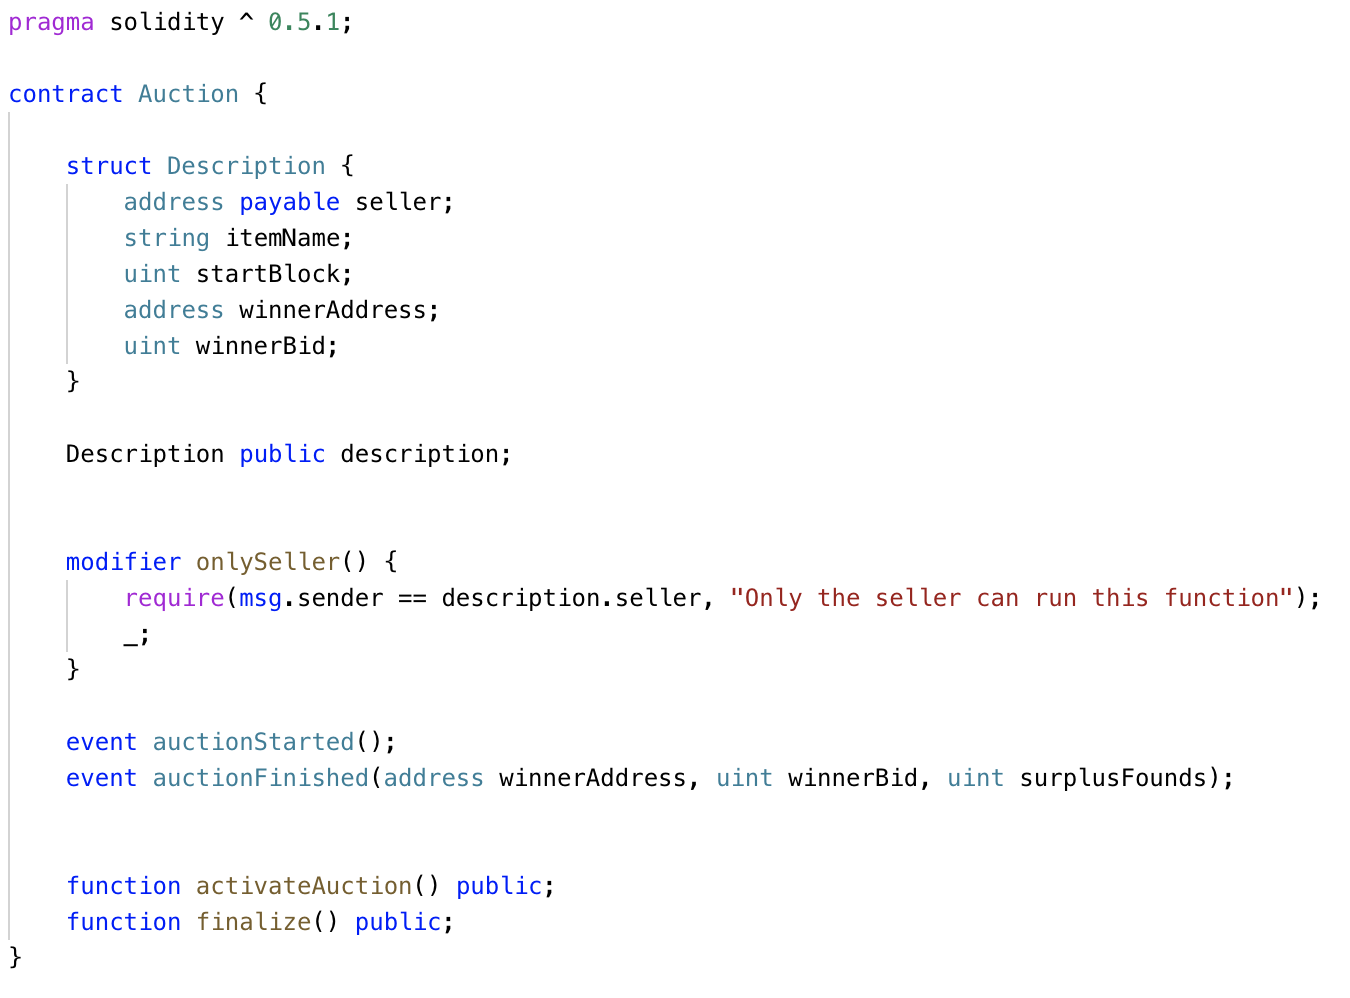
\includegraphics[width=\linewidth,]{images/auction.png}
\centering
\caption{Source code of \emph{Auction.sol}}
\label{fig:auction}
\end{figure}


\newpage
\section{DutchAuction.sol}
As specified in the requirements, the Dutch auction consists of an initial phase in which the price of the good is set to a very high price and afterwards, is gradually lowered by following a precise strategy. The auction finishes when someone is willing to pay the price of the good.

In this implementation of the Dutch auction, the contract extends the abstract contract \url{Auction} in order to  follow the \emph{Template-Method pattern} correctly and additionally, it uses a contract of class \url{Strategy} to implement the logic of devaluation.

\begin{figure}
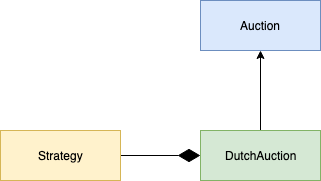
\includegraphics[width=140pt]{images/dutchUML.png}
\centering
\caption{UML view of \emph{DutchAuction}}
\label{fig:dutchUML}
\end{figure}



\newpage
\subsection{Strategy.sol \protect\footnote{Since every Dutch auction requires a strategy, we first describe the Strategy contract and afterwards the DutchAuction implementation.}}

We were asked to develop multiple method to compute the decrease of the price. In this work, this requirement has been developed exploiting an abstract contract (Figure \ref{fig:strategycode}) containing only one abstract method called \url{getPrice}.

\begin{figure}[h]
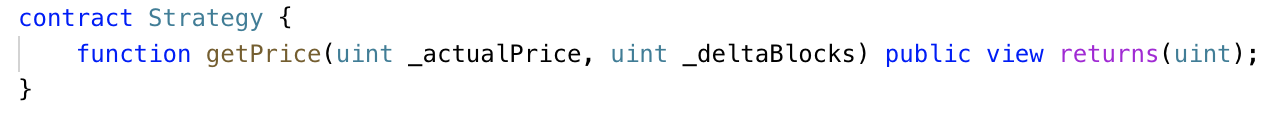
\includegraphics[width=\linewidth]{images/strategycode.png}
\centering
\caption{Source code of \emph{Strategy} abstract class}
\label{fig:strategycode}
\end{figure}

Afterwards, we create three sub-contracts implementing the \url{Strategy} contract, in order to let the user choice his own favorite strategy. In particular, \url{NormalStrategy} decreases in a linear way, then \url{SlowStrategy} decreases twice slower than \url{NormalStrategy} and finally, \url{FastStrategy} decreases twice faster than \url{NormalStrategy}.

\begin{figure}[h]
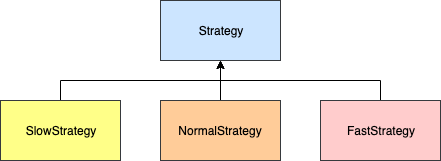
\includegraphics[width=220pt]{images/strategyUML.png}
\centering
\caption{UML view of the multiple \emph{Strategy}}
\label{fig:strategyUML}
\end{figure}

\newpage
\subsection{Status} \label{status}
Although in the Dutch auction there are only three explicit phases, for security reasons we added a new phase called \emph{Validation}. Since there could be the case in which two people make simultaneously a bid, as Figure \ref{fig:dutchStatus} shows, before closing the contract, we verify that at least 12 blocks \cite{ethBlog} have been confirmed. This restriction is essential to ensure that all miners own the same status of the contract and thus the same winner.

\begin{figure}[h]

\includegraphics[width=220pt]{images/dutchStatus.png}
\centering
\caption{Status of the \emph{Dutch} auction}
\label{fig:dutchStatus}
\end{figure}


\subsection{Constructor}
To create a new Dutch auction you need to insert the name of the item that you are willing to sold, both a reserve price and an initial price and lastly the address of a Strategy contract.

\begin{figure}[h]
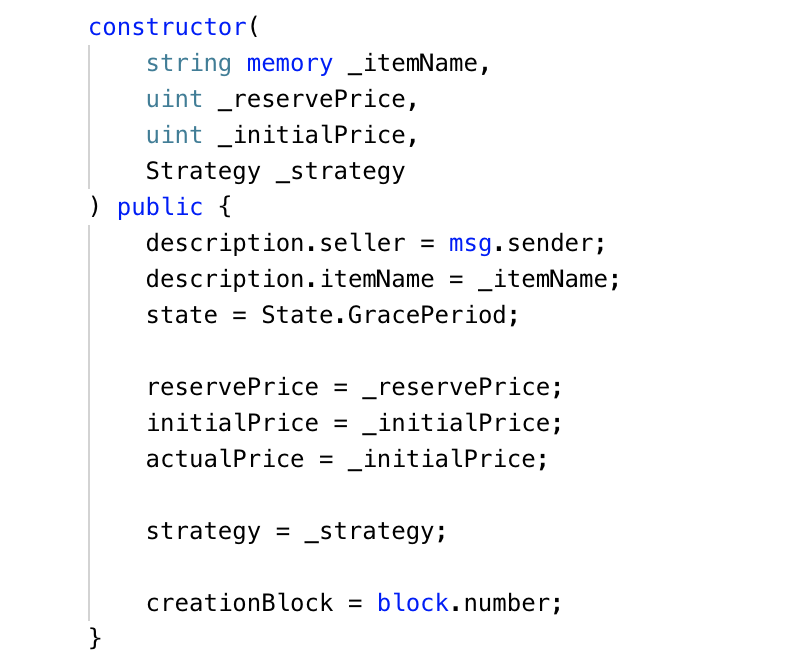
\includegraphics[width=0.6\linewidth]{images/DutchConstructor.png}
\centering
\caption{Source code of the \emph{DutchAuction} constructor}
\label{fig:dutchConstructor}
\end{figure}

Once deployed the contract correctly, its own status is set to \emph{Grace Period} . Note that in this implementation, the role of auctioneer does not exist and all critical functionalities are left to the seller of the item.

\newpage
\subsection{Functions}

\begin{figure}[h]
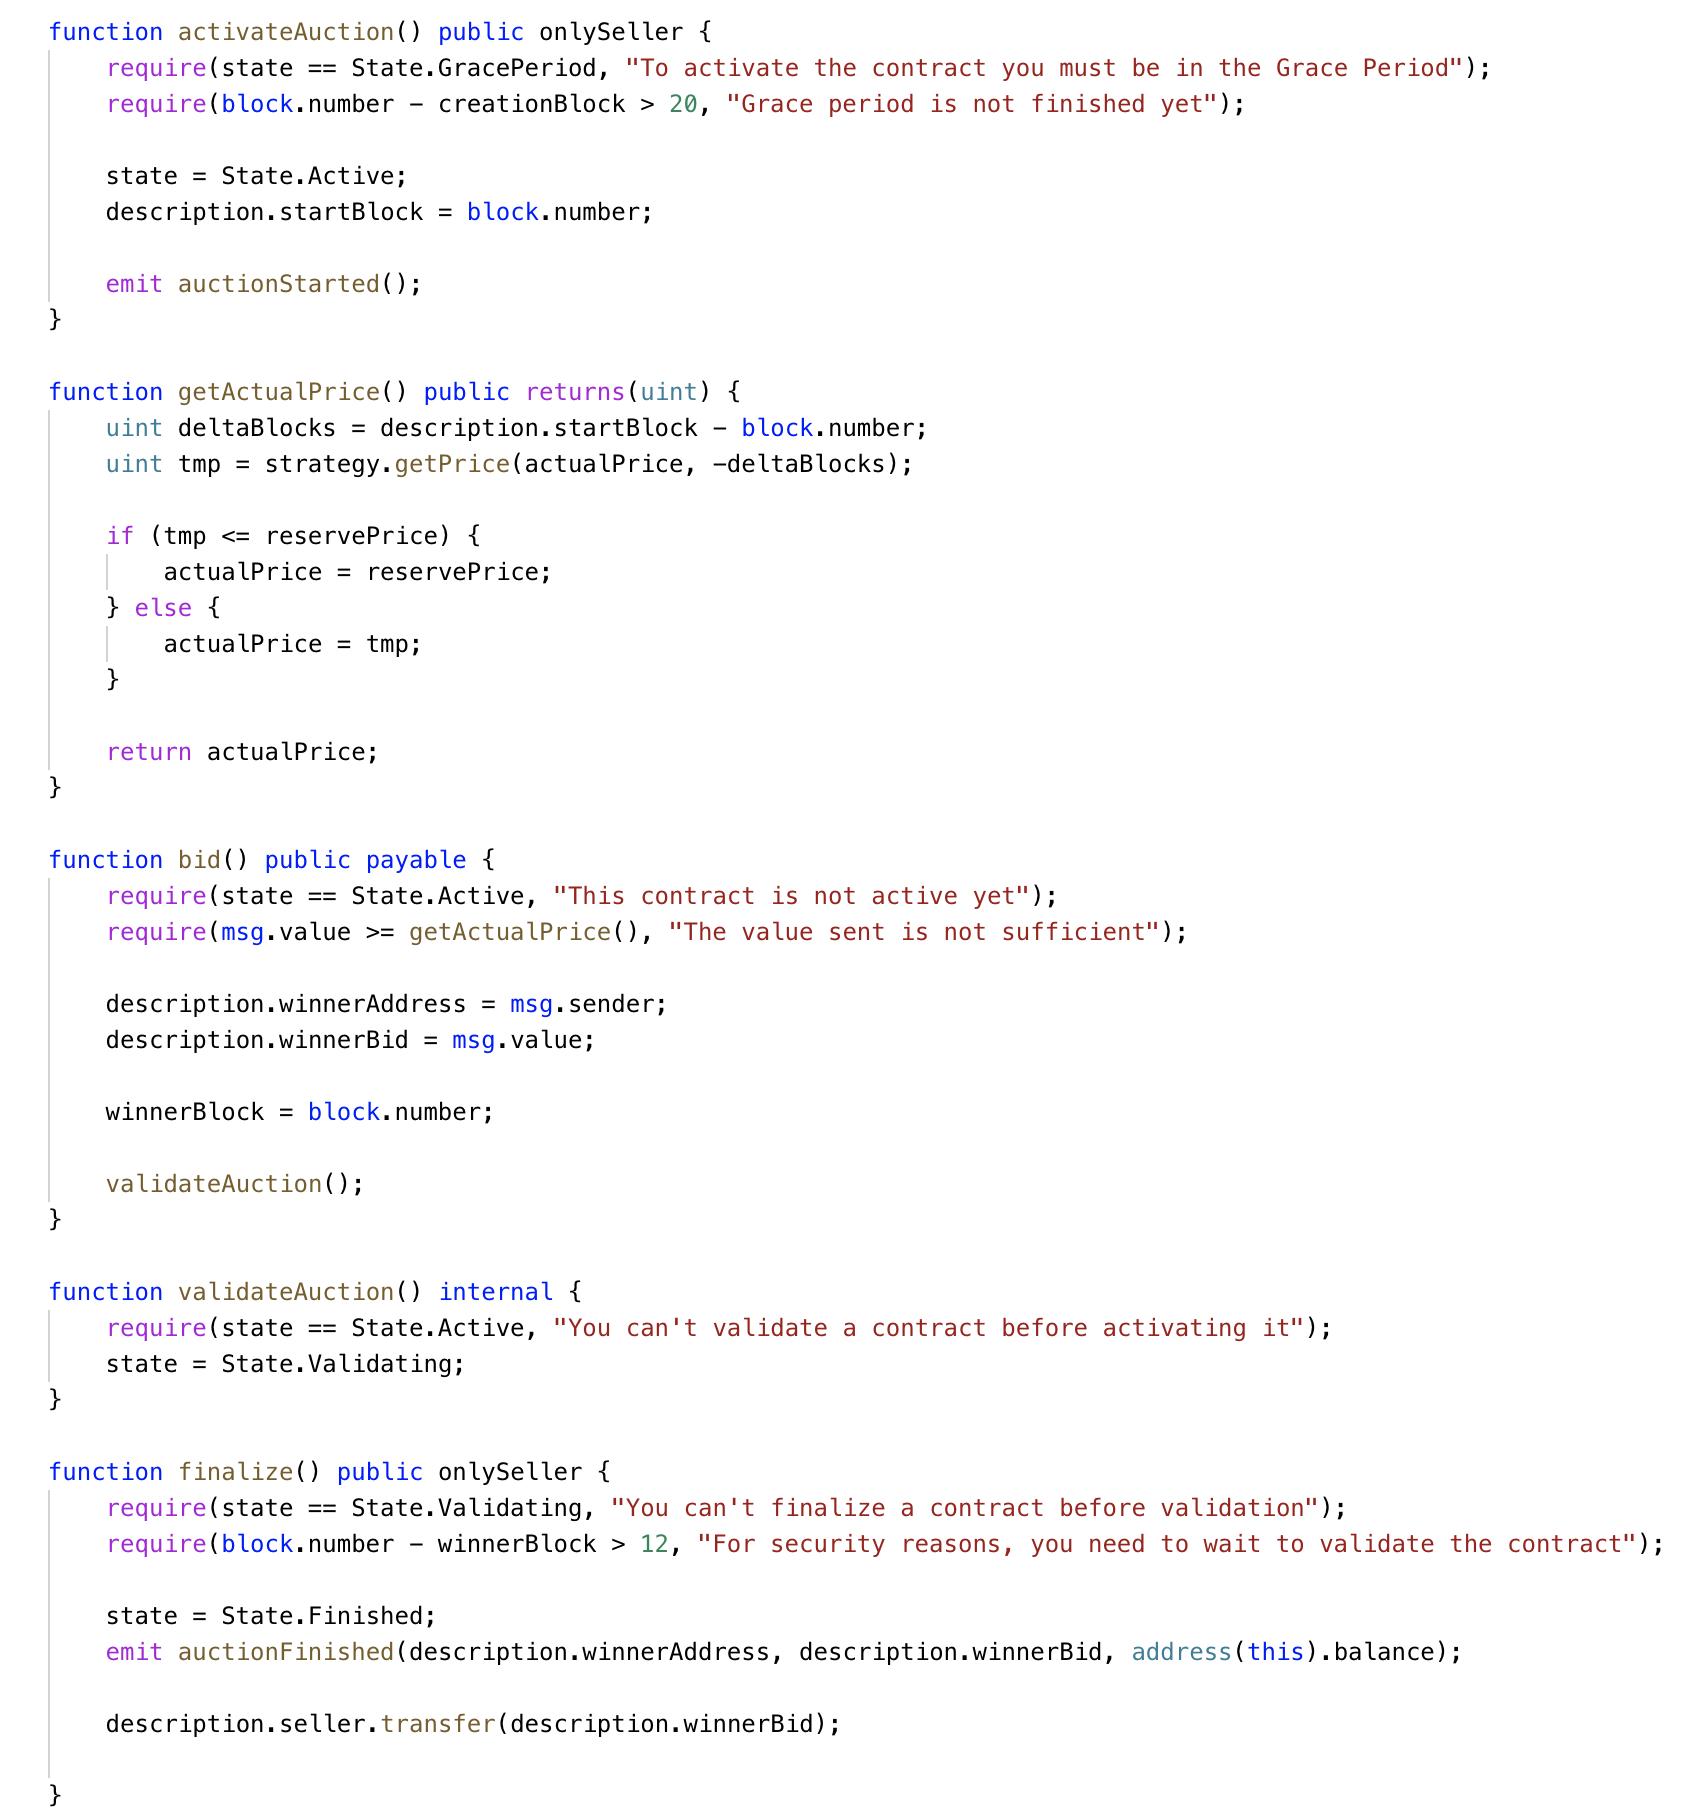
\includegraphics[width=\linewidth]{images/DutchCode.png}
\centering
\caption{Source code of the \emph{DutchAuction} functions}
\label{fig:DutchCode}
\end{figure}

To activate the auction, the \emph{Grace Period} of 5 minutes should finish. According to \url{etherscan}\cite{etherscan} every 15 seconds a new block is confirmed, hence:


\[5 \, min = 300 \, sec \implies \frac{300 \, sec}{15 \, sec/block}  = 20 \, blocks\]

By waiting 20 blocks we can (more or less) ensure the 5 minutes asked by the requirements.

Another interesting aspect is the \url{getActualPrice} function. Since the price drops over time, it must be updated, thus a public \url{uint} value on the blockchain is not sufficient. For this reason, people interested in knowing the price, should pay some gas to update the price. 

Now let's analyze the \url{bid} function. At the beginning of the function, we require that the \url{msg.value} (in other words, the money sent) are greater or equal the \url{actualPrice}. Right after this control, it is immediately written on the blockchain both the address of the user that made the bid, and the value of ether that he sent to the contract. Afterwards, due to security reasons related to simultaneous bids (as previously discussed in \ref{status}), the contract passes in a \emph{Validating} status. From now on, the seller can finalize the contract and receive the ether he's owed. 


\subsection{Gas Evaluation}

\begin{table}
\setlength{\tabcolsep}{10pt}
\setlength{\abovecaptionskip}{10pt}
\centering
\begin{tabular}{| c | c | c | c |} 
 \hline
 \textbf{Function} & \textbf{Transaction Cost} & \textbf{Execution Cost} & \textbf{Caller} \\
 \hline
 \emph{constructor} & 1067764 & 787072 & Seller \\ 
 \hline
 \url{activateAuction()} & 63359 & 42087 & Seller \\ 
 \hline
 \url{getActualPrice()} & 29677 & 8405 & All \\ 
 \hline
 \url{bid()} & 95839 & 74567 & All \\ 
 \hline
 \url{finalize()} & 37983 & 16711 & Seller \\
 \hline
 \hline
 \hline
 \textbf{\emph{Total}} & 1294622 & 928842 & \\ \hline
\end{tabular}
\caption{Gas consumption of \emph{DutchAuction} contract}
\label{table:1}
\end{table}



\newpage
\section{VickreyAuction.sol}
This kind of auction involves an initial phase in which all participants submit their bid in a sealed envelope. Afterwards, all these envelopes are opened and the person who did the highest bid, wins the auction by paying the second highest price. Due to possible fraud, people willing to submit their bid, must sent a deposit. This measure should discourage people in such unfair practices.

Similarly to the \url{DutchAuction}, the \url{VickreyAuction} as well extends the ``super-contract'' \url{Auction}, hence it inherits all the fields of its ``father''. Furthermore, in this way, the \emph{Template-Method pattern} is respected.  


\subsection{Phases}
The \url{VickreyAuction} starts with a \emph{Grace Period} of 5 minutes in the same way of the \url{DutchAuction}. The second phase called \emph{Commitment}, is the period in which people can submit their bids. The novelty is the \emph{Withdrawal} phase. Basically, during this phase the bidders can withdrawn their bids and get only half of their deposit back. Then we have the \emph{Opening} phase, that is the period in which all the bids are opened, and lastly the closing of the contract.

\begin{figure}[h]

\includegraphics[width=0.9\linewidth]{images/vickreyPhases.png}
\centering
\caption{Phases of the \emph{Vickrey} auction}
\label{fig:dutchConstructor}
\end{figure}


\subsection{Constructor}
To create a Vickrey auction, few parameters are needed. In particular, the lengths of all the phases are required, as well as both the reserve price and the minimum deposit. Note from Figure \ref{fig:vickreyConstructor} that in this implementation, the minimum deposit must be greater or equal to the reserve price.



\begin{figure}[h]
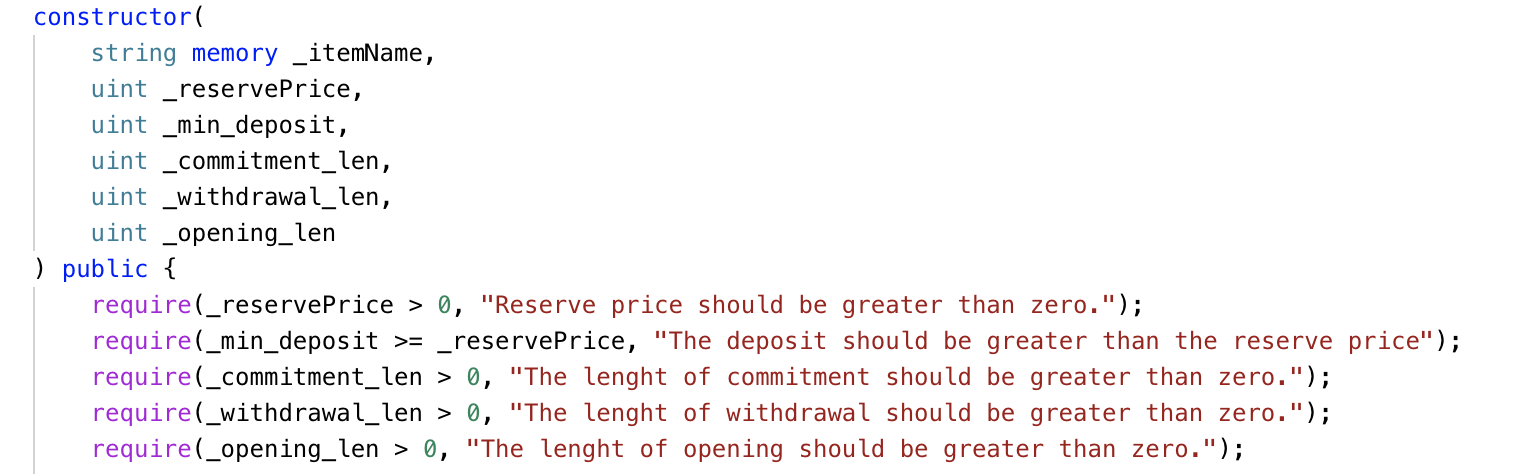
\includegraphics[width=\linewidth]{images/vickreyConstructor.png}
\centering
\caption{Source code of \emph{VickreyAuction} constructor}
\label{fig:vickreyConstructor}
\end{figure}


\newpage
\subsection{GenerateBid.sol}\label{genbid}
To help people in making bids, we create a contract called \url{GenerateBid}. As you can see from Figure \ref{fig:GenerateBid}, there is a function called \url{generateBid}, that given an integer value in input (the desired bid), it returns a 32-bit nonce obtained from the timestamp, and also the hash of the tuple \(<bid \, , nonce>\). Of course, it will be the responsibility of the person who did the bid, not to reveal neither his bid nor his nonce.

\begin{figure}[h]
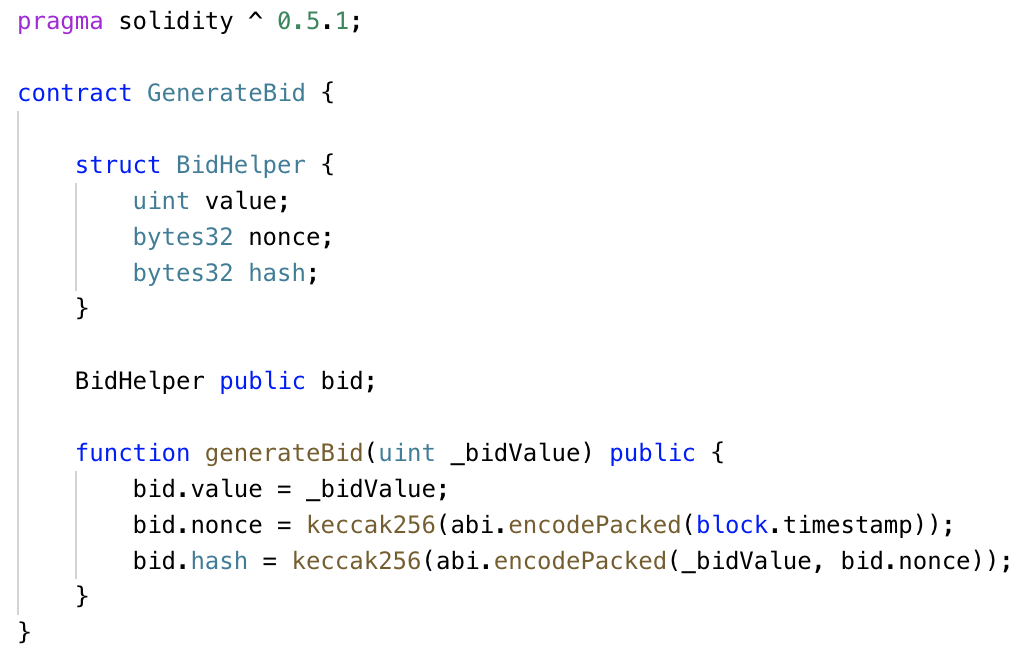
\includegraphics[width=0.7\linewidth]{images/generateBid.png}
\centering
\caption{Source code of \emph{GenerateBid} contract}
\label{fig:GenerateBid}
\end{figure}




\newpage
\subsection{Modifiers}
Before going deeper in the function implementations, we need first to understand the modifiers declared inside the contract. This tool (the modifier), allow to execute some code before and after a function. In particular, the code of the function will be executed when the \url{_;} symbols will occur.

By exploiting the potentialities of modifiers, we defined a way to control whether the actual phase is the one desired.


\begin{figure}[h]
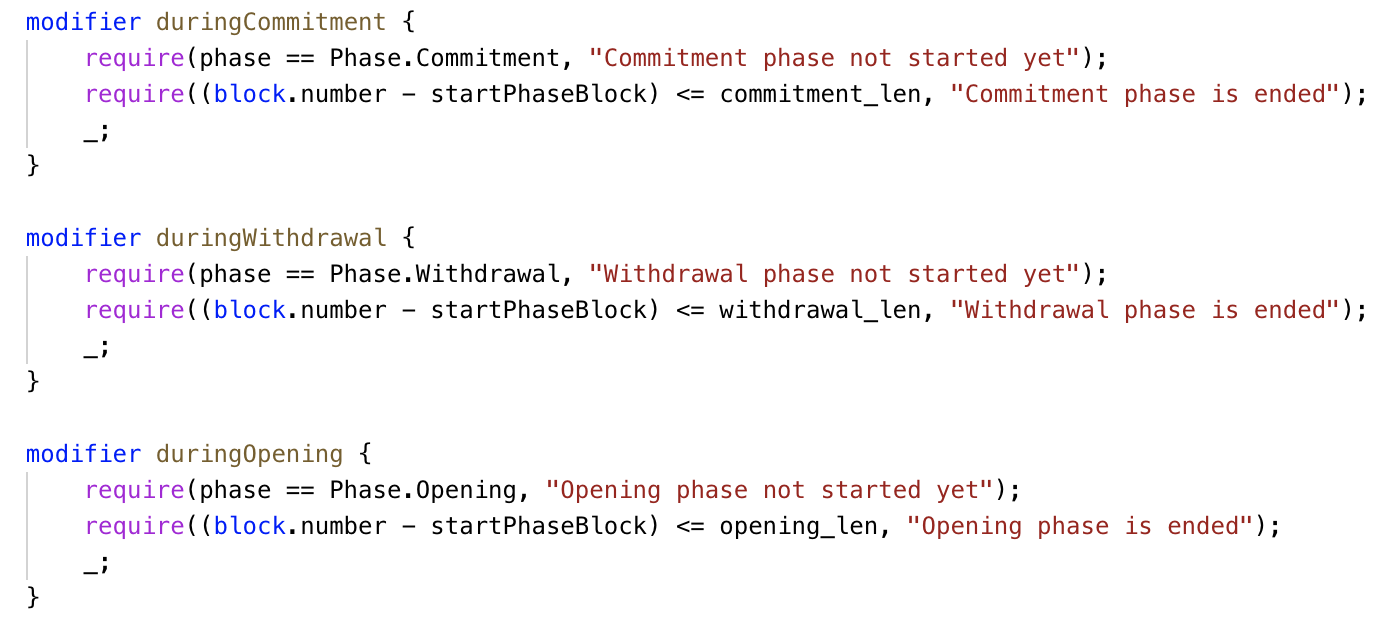
\includegraphics[width=\linewidth]{images/vickreyModifier.png}
\centering
\caption{Source code of \emph{VickreyAuction} modifiers}
\label{fig:vickreyModifiers}
\end{figure}


\subsection{Commitment}
As already explained in Section \ref{genbid} every \url{bid} is composed by three parameters:
\begin{enumerate}
\item the \url{uint} value of the bid;
\item a \url{bytes32} nonce;
\item the hash of \(<bid \, , nonce>\).
\end{enumerate}
Now, since the bids must be secret until the opening phase, the contract should not write any information about these bids on the blockchain. To make it possible, the function requires and stores only the hash. In this way, only during the opening phase, we require both the value and the nonce, in order to verify the hash and thus the correctness of the bid. 

Of course, to avoid misbehavior, people have to submit a deposit greater or equal the minimum deposit decided at deploy time by the seller.

Note that all these bids are stored in a non-public \url{mapping(address => Bid)} called \emph{bids}.

\begin{figure}[h]
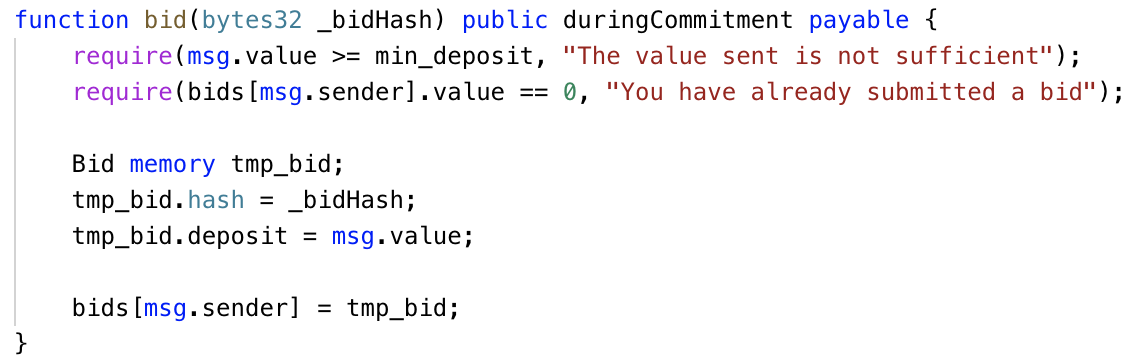
\includegraphics[width=\linewidth]{images/bid.png}
\centering
\caption{Source code of \emph{bid} function}
\label{fig:vickreyBid}
\end{figure}


\newpage
\subsection{Withdrawal}
Another interesting aspect of the Vickrey auction, is the \emph{Withdrawal} phase. During this period of time, people can retire their bids, but only half of the deposit will be reimbursed. 

As Wohrer et al. \cite{soliditypattern} suggest, when a contract calls another contract,  it  hands  over  control  to  that other  contract.  The  called  contract  can then, in turn, re-enter the contract by which it was called and try to manipulate its state or hijack the control flow through malicious code. A solution is the \emph{Checks-Effects-Interaction pattern}. Basically, all the calls to external contracts, are always placed at the end of the function. This way, the possible attack surface is limited. 

This pattern is divided in three phases: first, check all the preconditions, then make changes to the contract’s state, and finally interact with other contracts.

\begin{figure}[h]
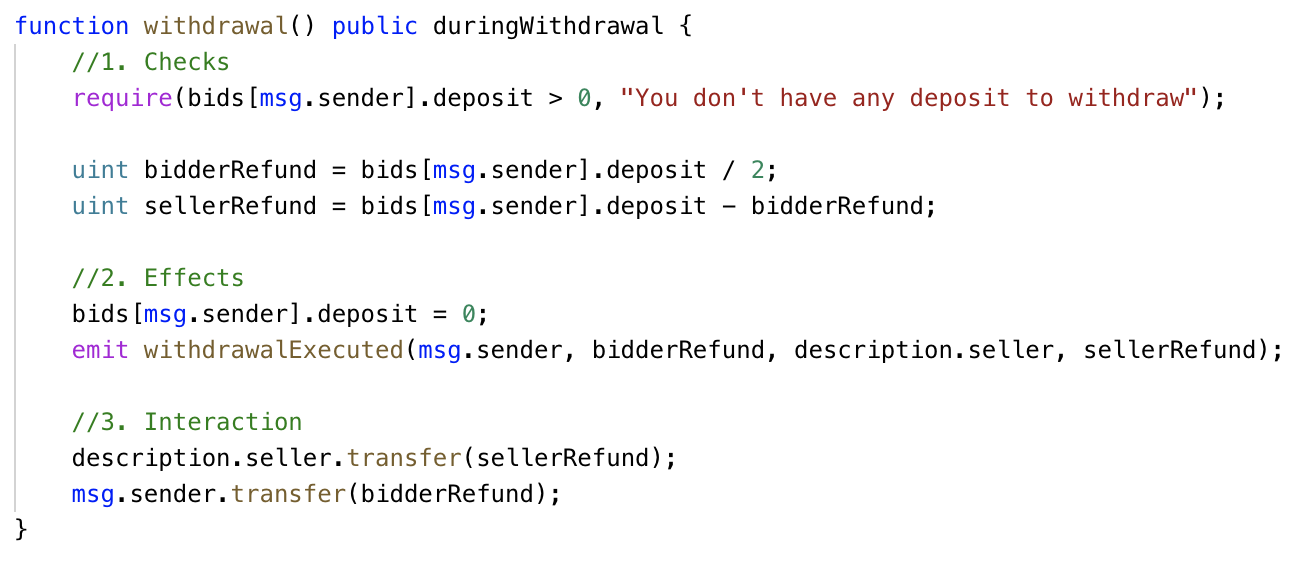
\includegraphics[width=\linewidth]{images/withdrawal.png}
\centering
\caption{Source code of \emph{withdrawal} function}
\label{fig:vickreyWith}
\end{figure}


\newpage
\subsection{Opening}
As written in the requirements, in the opening phase all bidders should reveal their bid by sending the nonce used previously. At the top of Figure \ref{fig:vickreyOpen}, we can see that the only parameter required by the \url{open} function is a \url{bytes32} nonce. If bidders used our generator (see \ref{genbid}), this nonce value can be easily pasted and sent to the contract. The first control that is done, is the correctness of the hash previously sent, by checking the hash of the tuple \(<bid \, , nonce>\). If this constraint is respected, then the bidder can be refunded. Afterwards, we check whether the current bid is the first or not, and then by looking at the value sent, we declare the winner and the highest second bid. Note that in case of overwriting of the winner, there is a refund the old highest bidder.

\begin{figure}[h]
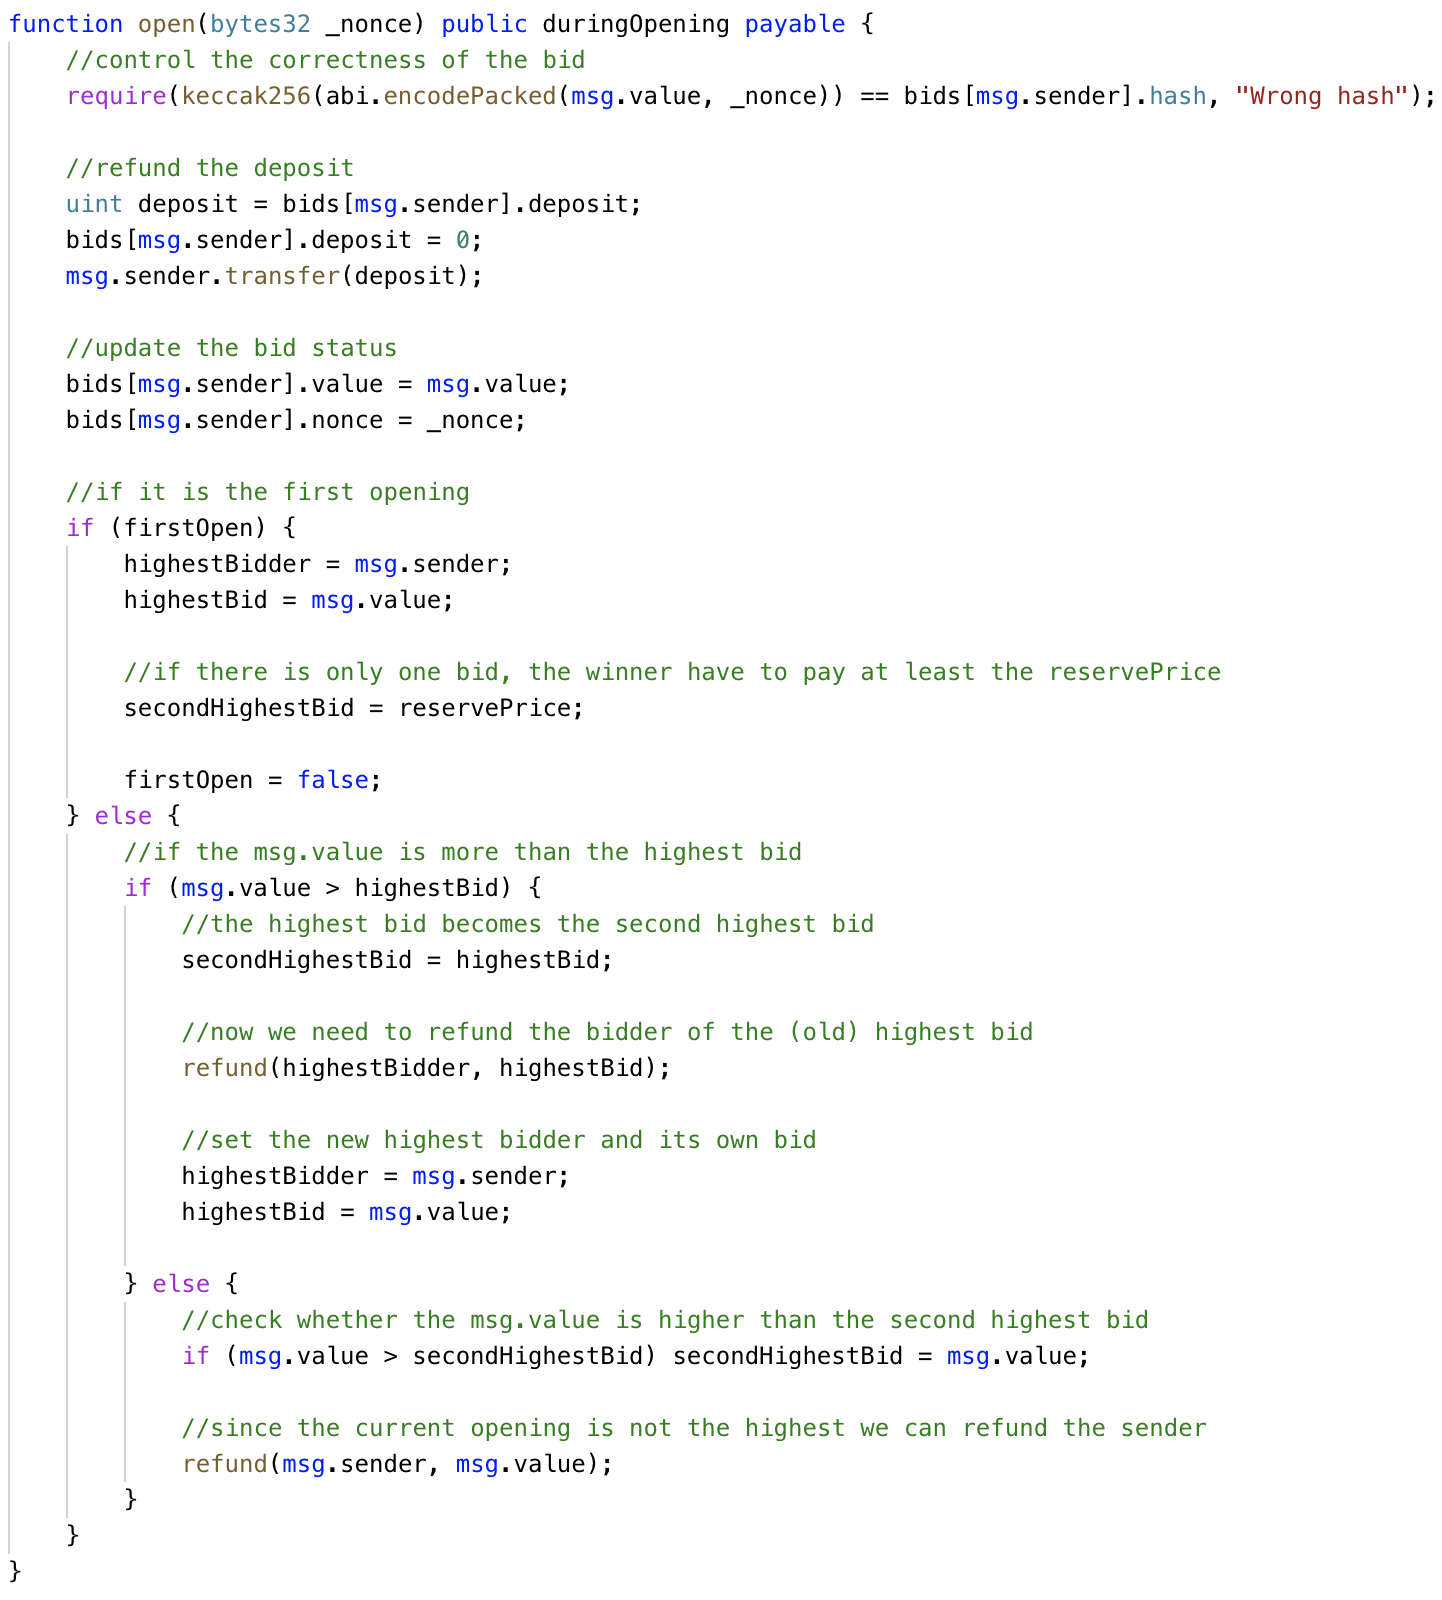
\includegraphics[width=0.92\linewidth]{images/opening.png}
\centering
\caption{Source code of \emph{open} function}
\label{fig:vickreyOpen}
\end{figure}


\newpage
\subsection{Finalize}
This function is the last step before closing definitely the contract. If there is at least a bid, or in other words, if there is a winner, we refund him with the difference between his bid and the second highest. Afterwards we close the auction, we send money to the seller and if there is a surplus (for instance someone who sent a bid, but forgot to opening it), we transfer this money to a charity address.

\begin{figure}[h]
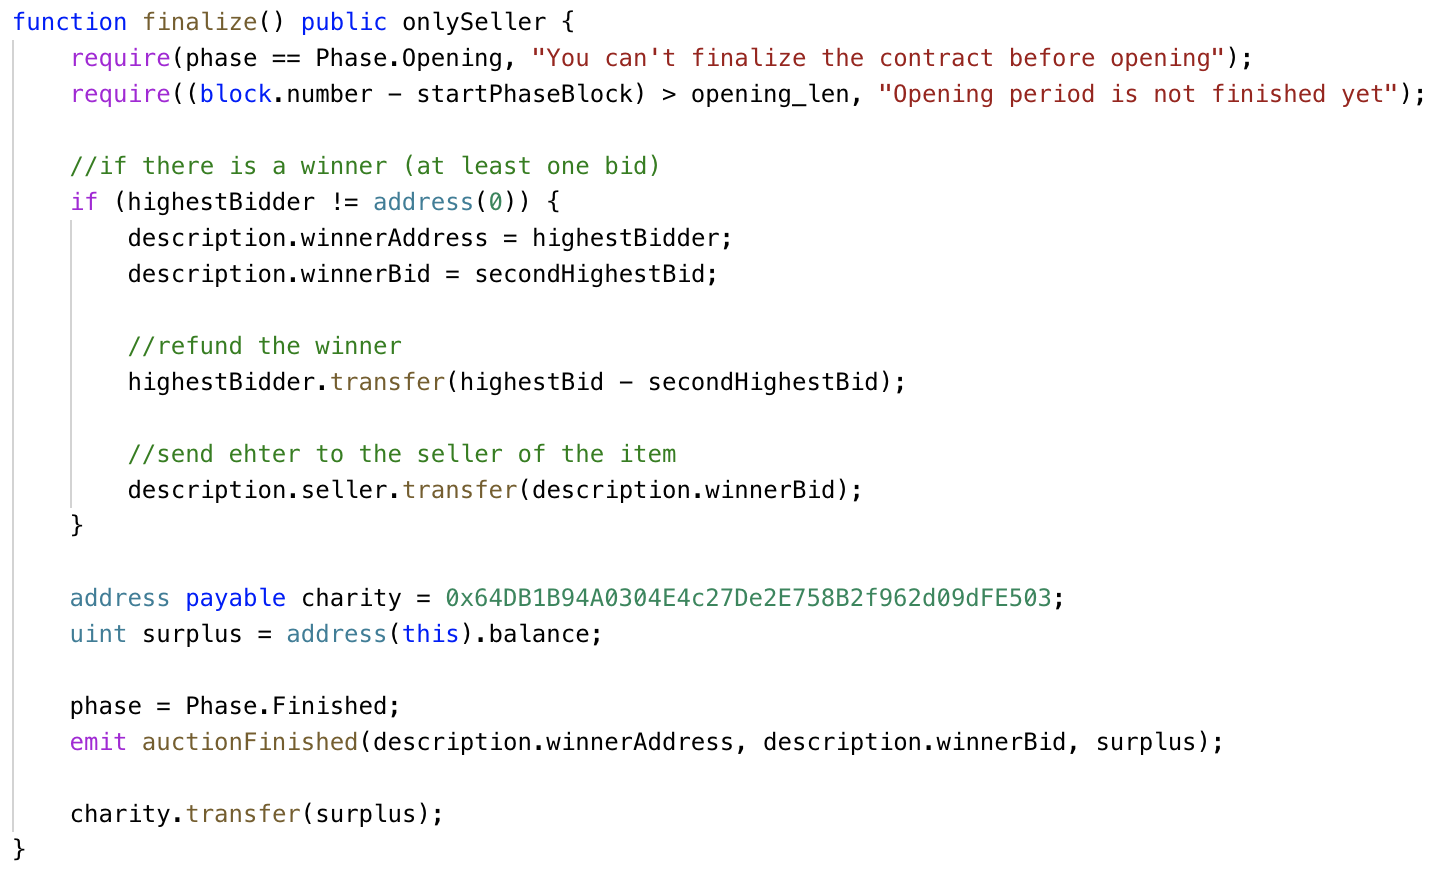
\includegraphics[width=0.85\linewidth]{images/finalize.png}
\centering
\caption{Source code of \emph{finalize} function}
\label{fig:vickreyFinalize}
\end{figure}


\subsection{Gas Evaluation}

\begin{table}
\setlength{\tabcolsep}{10pt}
\setlength{\abovecaptionskip}{10pt}
\centering
\begin{tabular}{| c | c | c | c |} 
 \hline
 \textbf{Function} & \textbf{Transaction Cost} & \textbf{Execution Cost} & \textbf{Caller} \\
 \hline
 \emph{constructor} & 2226512 & 1664784 & Seller \\ 
 \hline
 \url{activateAuction()} & 68350 & 47078 & Seller \\ 
 \hline
 \url{bid()} & 65790 & 42342 & All \\ 
 \hline
 \url{startWithdrawal()} & 33619 & 12347 & Seller \\
 \hline
 \url{withdrawal()} & 30811 & 24539 & All \\
 \hline
 \url{startOpening()} & 33685 & 12413 & Seller \\
 \hline
 \url{open()} & 114170 & 120722 & All \\
 \hline
 \url{finalize()} & 119843 & 98571 & Seller \\
 \hline
 \hline
 \hline
 \textbf{\emph{Total}} & 2578610 & 2022796 & \\ \hline
\end{tabular}
\caption{Gas consumption of \emph{VickreyAuction} contract}
\label{table:2}
\end{table}


\newpage
\begin{thebibliography}{4}

\bibitem{ethBlog} Ethereum Blog, 
\url{https://blog.ethereum.org/2015/09/14/on-slow-and-fast-block-times}

\bibitem{etherscan} Block Explorer and Analytics Platform for Ethereum, 
\url{https://etherscan.io/chart/blocktime}

\bibitem{soliditypattern}
Wohrer, Maximilian, and Uwe Zdun. "Smart contracts: security patterns in the ethereum ecosystem and solidity." 2018 \emph{International Workshop on Blockchain Oriented Software Engineering (IWBOSE)}. IEEE, 2018.


\end{thebibliography}

\end{document}